
3D visualizers allow the user to visualize the data sets as three dimensional models and work with them in the three dimensional space.

\subsection{Isosurface}

The isosurface visualizer supports the visualization of a data set as an isosurface. Isosurfaces are
surfaces in data sets with equal density. This allows displaying structures of
similar or equal density as a solid object.
The Isosurface Visualizer supports viewing the objects, manipulating the data set's position and rotation, and performing simple geometrical measurements.

\subsubsection{Selected data set}
The Selected data set panel shows the currently selected data set. The selection can be changed by choosing a different data set from the dropdown list.
The currently selected data set is the data set that is chosen as target for specific mouse operations and other actions.
The selected data set is also highlighted in the 3D scene having an orange colored bounding box.
The option \emph{Hide} allows to hide the the data set in the rendered scene.

\begin{figure}[h!]
  \centering
  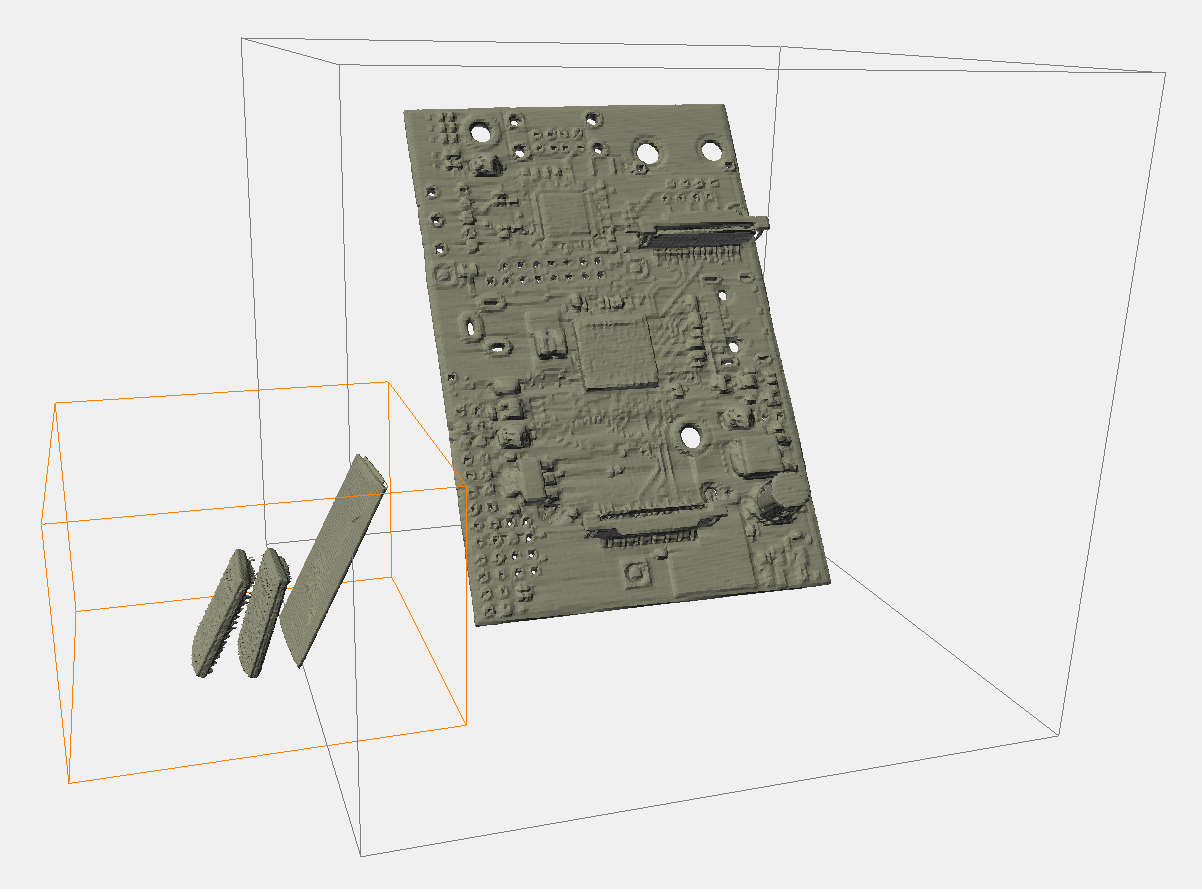
\includegraphics[width=0.75\textwidth]{img/selecteddataset.png}
  \caption{An Isosurface with two loaded data sets. The left data set is selected as indicated by the orange color of the bounding box.}
\end{figure}

\subsubsection{Mouse Operation}\label{sec:mouseoperation}
The Mouse Operation panel determines how mouse clicks and mouse drags (press mouse button + move) are interpreted.

Each switch button represents a specific mouse operation. Only one switch button can be activated at the same time. Activating a button
deactivates all other buttons. If no button is activated, the default mouse operation \emph{Rotate View} is active
(see \fullref{sec:isocontrols}).
The panel contains the following switch buttons:

\begin{itemize}
  \item{\emph{Move}\newline Dragging the mouse in the view adjusts the position of the currently selected data set.
  If no data set is selected the data set the mouse is pointing at is automatically selected.}
  \item{\emph{Rotate}\newline Dragging the mouse in the view adjusts the rotation of the currently selected data set.
  If no data set is selected the data set the mouse is pointing at is automatically selected.}
  \item{\emph{Select}\newline Mouse clicks result in a select operation. The data set the mouse cursor is pointing at is selected.
  If the mouse cursor does not point at an object, the currently selected object is deselected.}
  \item{\emph{Add point}\newline Adds a data point at the position the mouse cursor is pointing at.
  The newly added data point is assigned to the data set that touches this point.
  This data set is also automatically activated and selected.}
\end{itemize}

Pressing the middle mouse button while moving the mouse automatically results in a \nameref{par:rotate_view} operation, regardless of what switch button is activated.\newline
Holding CTRL while moving the mouse automatically results in a \nameref{par:move_view} operation, regardless of what switch button is pressed.

\paragraph{Axis filter}
If \emph{Move} or \emph{Rotate} is activated, there is also an additional section that allows to filter the movements.
The X-,Y- and Z-buttons determine how the selected object is moved or rotated. For example if only the Z-button is activated,
object movements are only performed on the Z-axis while in rotation mode objects are rotated arround the Z-axis. The button \emph{Slice} activates
the slice mode. If this button is activated, all moving and rotation operations are instead applied to the slice that is selected in the
\nameref{sec:slicemanagement} panel.

\subsubsection{Object Properties}

In this section current selected object properties can be viewed and edited. The object responds in real time by entering in the textfields. The representation of rotation has two modes. The rotation representation of the objct can be switched beteween quaternion or euler angles by clicking on the \textit{Rotation Mode} button.

\subsubsection{Camera Properties}

The camera properties contains the rotation of the camera and the current relative zoom. The camera responds in real time by entering in the textfields. The Rotatin can be switched like the object properties.

\subsubsection{Render Settings}
The Isosurface visualizer can be set up via its side panel section.
The section has multiple options:
\begin{itemize}
  \item{\emph{Threshold}\newline The threshold value for the isosurface.}
  \item{\emph{Method}\newline The method used for generating the isosurface.}
  \item{\emph{Invert}\newline A flag that determines if the surface is built
    against values below the threshold or above the threshold.}
  \item{\emph{Refresh}\newline Refreshes the isosurface model.}
  \item{\emph{Projection}\newline Perspective projection is active by default, 
  orthographic projection can be activated with this checkbox.}
  \item{\emph{Views}\newline Immediately snaps the camera to a fixed viewing angle.}
\end{itemize}
The Isosurface visualizer needs some time to generate an isosurface so it does not
view anything by default.
The visualizer needs to be set up and then the \emph{Refresh}-Button must be pressed
to regenerate the isosurface model.

\subsubsection{Slice Management}\label{sec:slicemanagement}
The Slice Management Panel allows to select slices, setup the voxel output of a slice, or define one or multiple \nameref{sec:def_cuttingplane}.
The panel contains the following sections:
\begin{itemize}
  \item{\emph{Selected Slice}\newline Displays a list of all slices that are loaded into the Isosurface Visualizer.
  A slice can be selected by choosing it from the list. This slice is then selected as the currently active slice and
  can be setup as cutting plane, moved and rotated in the view (see \fullref{sec:mouseoperation}). To recognize the selected slice in the 3D Scene it is displayed with a slightly more intense color than other slices.
  in the Isosurface View.}
  \item{\emph{Data set}\newline Displays the name of the dataset the currently selected slice belongs to.}
  \item{\emph{Display Voxel Slice}\newline Shows or hides the voxel slice output on the current slice (see \autoref{fig:iso_voxel_slice}).}
  \item{\emph{Resolution}\newline Sets the output resolution of the voxel output texture that is projected onto the
  currently selected slice (see \autoref{fig:iso_voxel_slice}).
  Higher resolutions show more details, but slow down the PC performance.}
  \item{\emph{Colorizer}\newline The colorizer is only visible if the checkbox \emph{Display Voxel Slice} is checked.
  If so, the user can set color mappings just like in the Slice Visualizer (See \fullref{sec:Colorizer}).
  Note that each slice has its own colorizer settings.}
  \item{\emph{Cutting Direction}\newline If a slice is selected, the dropdown list shows the cutting direction of this slice.
  To change the cutting direction, the user can select a different cutting direction from the list.
  The cutting direction determines which part of the surface is cut away.
  If the camera view is in default mode and neither the slice nor the dataset was rotated, \emph{Positive} cuts away
  the front part of the dataset while \emph{Negative} cuts away the back part.}
  \item{\emph{Cutting Mode}\newline Supports a custom setting to determine how the parts of an data set with multiple
  cutting planes are displayed. Normally a cutting plane cuts away the complete back or front part of an surface.
  But if multiple cutting planes are set up for the same data set, custom settings are possible like hiding only parts that are cut
  away by at least two slices or hiding parts that are cut away by all slices except for a specific number.
  The dropdown list that is followed by the text \emph{Hide parts that are cut out by} has two options.\newline
  The first option, \emph{at least}, is the default option and hides away all parts that are
  cut out by at least the amount of cutting planes that is specified in the text box. For example
  if \emph{at least} is selected and 2 is entered in the text box, only those parts of the surface are hidden that are cut out by
  at least two cutting planes.\newline
  The second option \emph{all but} determines that only parts are hidden that are cut out by all minus the specified number of cutting planes.
  For example if this mode is selected and the default value 0 is entered in the amount box, only those parts are hidden that are cut out
  by all slices.}
\end{itemize}

\begin{figure}[h!]
  \centering
  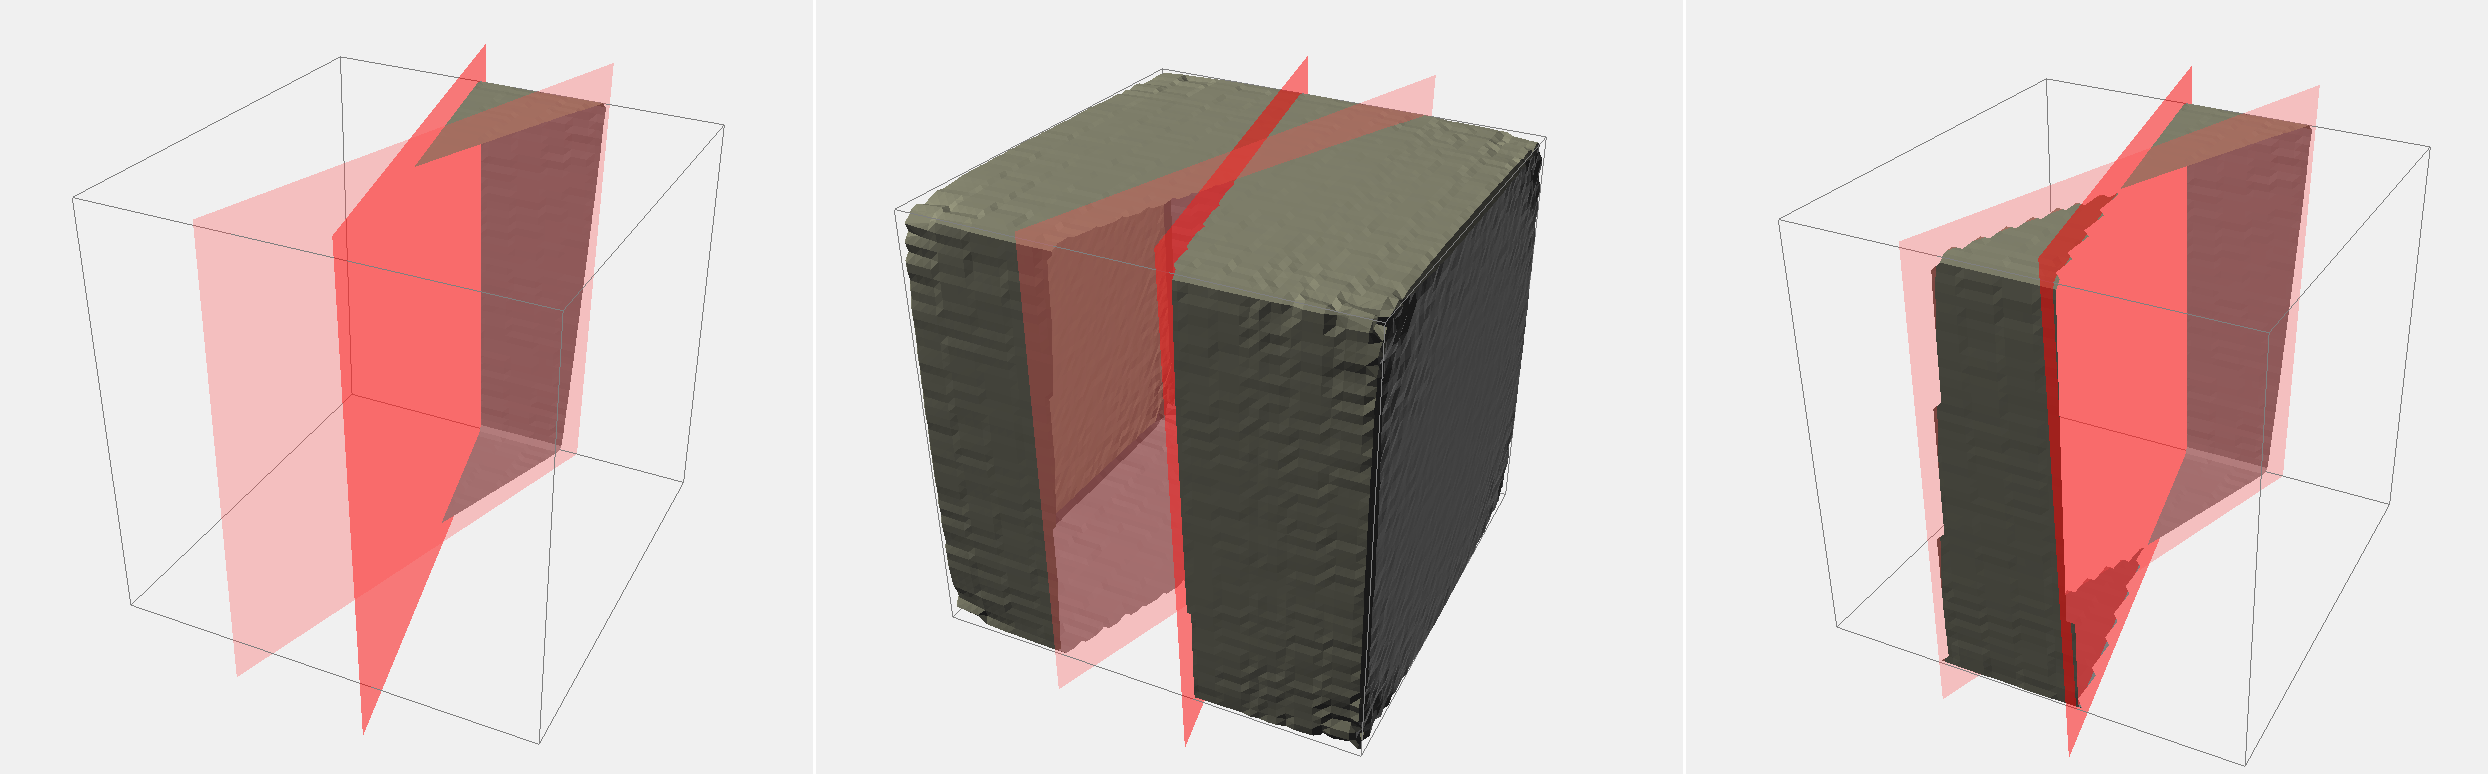
\includegraphics[width=1.0\textwidth]{img/cuttingplane_modes.png}
  \caption{An isosurface cube with two cutting planes rendered with different cutting modes.\newline
  Left: Default cutting mode \emph{at least 1} hides all parts that are cut out by at least one cutting plane.\newline
  Center: Cutting mode \emph{at least 2} hides all parts that are cut out by both planes.
  \newline
  Right: Cutting mode \emph{all but 1} hides all parts that are cut out by all but one, in this case exactly one cutting plane.}
  \label{fig:cuttingplane_modes}
\end{figure}

\begin{figure}[h!]
  \centering
  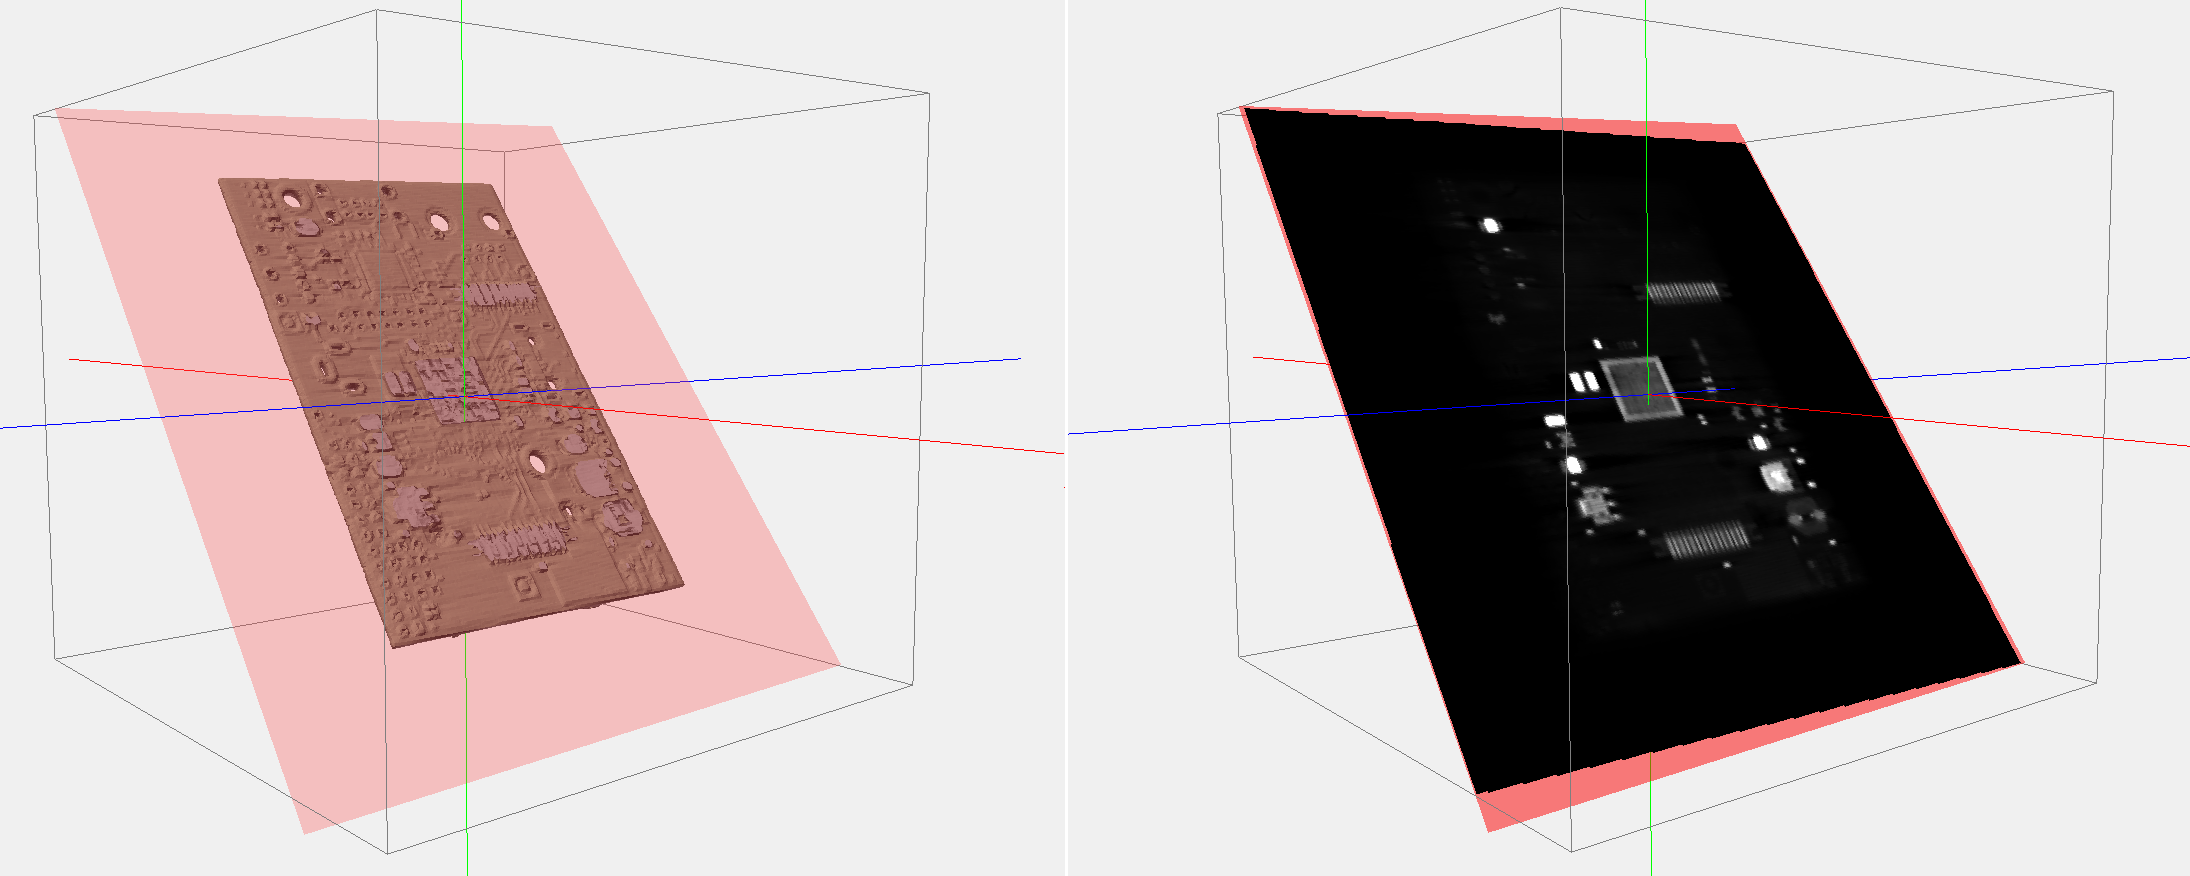
\includegraphics[width=1.0\textwidth]{img/iso_voxel_slice.png}
  \caption{The isosurface of a Raspberry Pi.\newline
  The left image shows a cutting plane cutting out the upper part of the Raspberry Pi.\newline
  The right image shows the same cutting plane but the voxels on the slice are projected onto the 3D slice.}
  \label{fig:iso_voxel_slice}
\end{figure}

\paragraph{Remarks}
In \autoref{fig:cuttingplane_modes} you can see that some parts of the surface have unsharp edges. This happens if a none default cutting mode
is applied. As result parts that are normally hidden by default are forced to be visible. This is done by setting the distance of a rendered point
to a value indicating that this point is not cut away. For simplicity, this value is not calculated exactly and a default value is taken - this leads to unsharp
edges for those enforced visible parts.

\subsubsection{GeometricAnalysis}
This section works very similarly to its equivalent in the slice view (see \fullref{sec:2dGeometricAnalysis}).

\subsubsection{Grid}

This grid is builded up like the grid in the slice visualizer. This section allows you to place a grid in the 3D-Room of the isosurface. The color, opacity and mesh width can be change via colorpicker, slider and direct text input. In addition, the mode of the grid can be switched. Selectable modes are fixed and automatic. In the fixed mode, the grid has exactly the entered mesh width and does not change. In the automatic mode, on the other hand, the mesh width adjusts so that the grid always remains visible.


\subsubsection{Controls}\label{sec:isocontrols}
\paragraph{Rotate View}\label{par:rotate_view}
The camera view can be rotated by moving the mouse over the visualizer window while
holding down the left mouse button or the middle mouse button.

\paragraph{Move View}\label{par:move_view}
Holding CTRL and the left mouse button while moving the mouse moves the point the camera is looking at.

\paragraph{Zoom}
Scrolling the mouse wheel will zoom in or out the view.

\subsubsection{Adding datasets}
Additional datasets can be added to an Isosurface View by right clicking on the entry of that \emph{Isosurface}
in the \emph{Data Objects} Tree in the side panel and choosing the operation \emph{Add dataset} as seen in \autoref{fig:adddataset}.
After choosing that action a dialog appears that shows all available data sets. Select the data set you want to add and click \emph{OK}.
The data set is then loaded to the selected Isosurface.

\begin{figure}[h!]
  \centering
  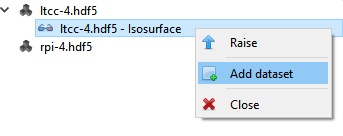
\includegraphics[width=0.5\textwidth]{img/adddataset.png}
  \caption{Adding a data set the to an Isosurface}
  \label{fig:adddataset}
\end{figure}

\begin{figure}[h!]
  \centering
  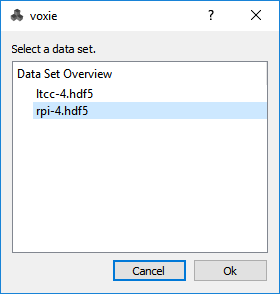
\includegraphics[width=0.5\textwidth]{img/adddataset_dialog.png}
  \caption{Choose the data set that should be added to the isosurface}
\end{figure}

\subsubsection{Restriction of the zoom}\label{restrictionOfTheZoom}

This module limits the zooming out and zooming in of an object.
The minimum zoom is 0\%. It can not be further zoomed out. This way the object can
never be lost and it is always found again.

\begin{figure}[h!]
  \centering
  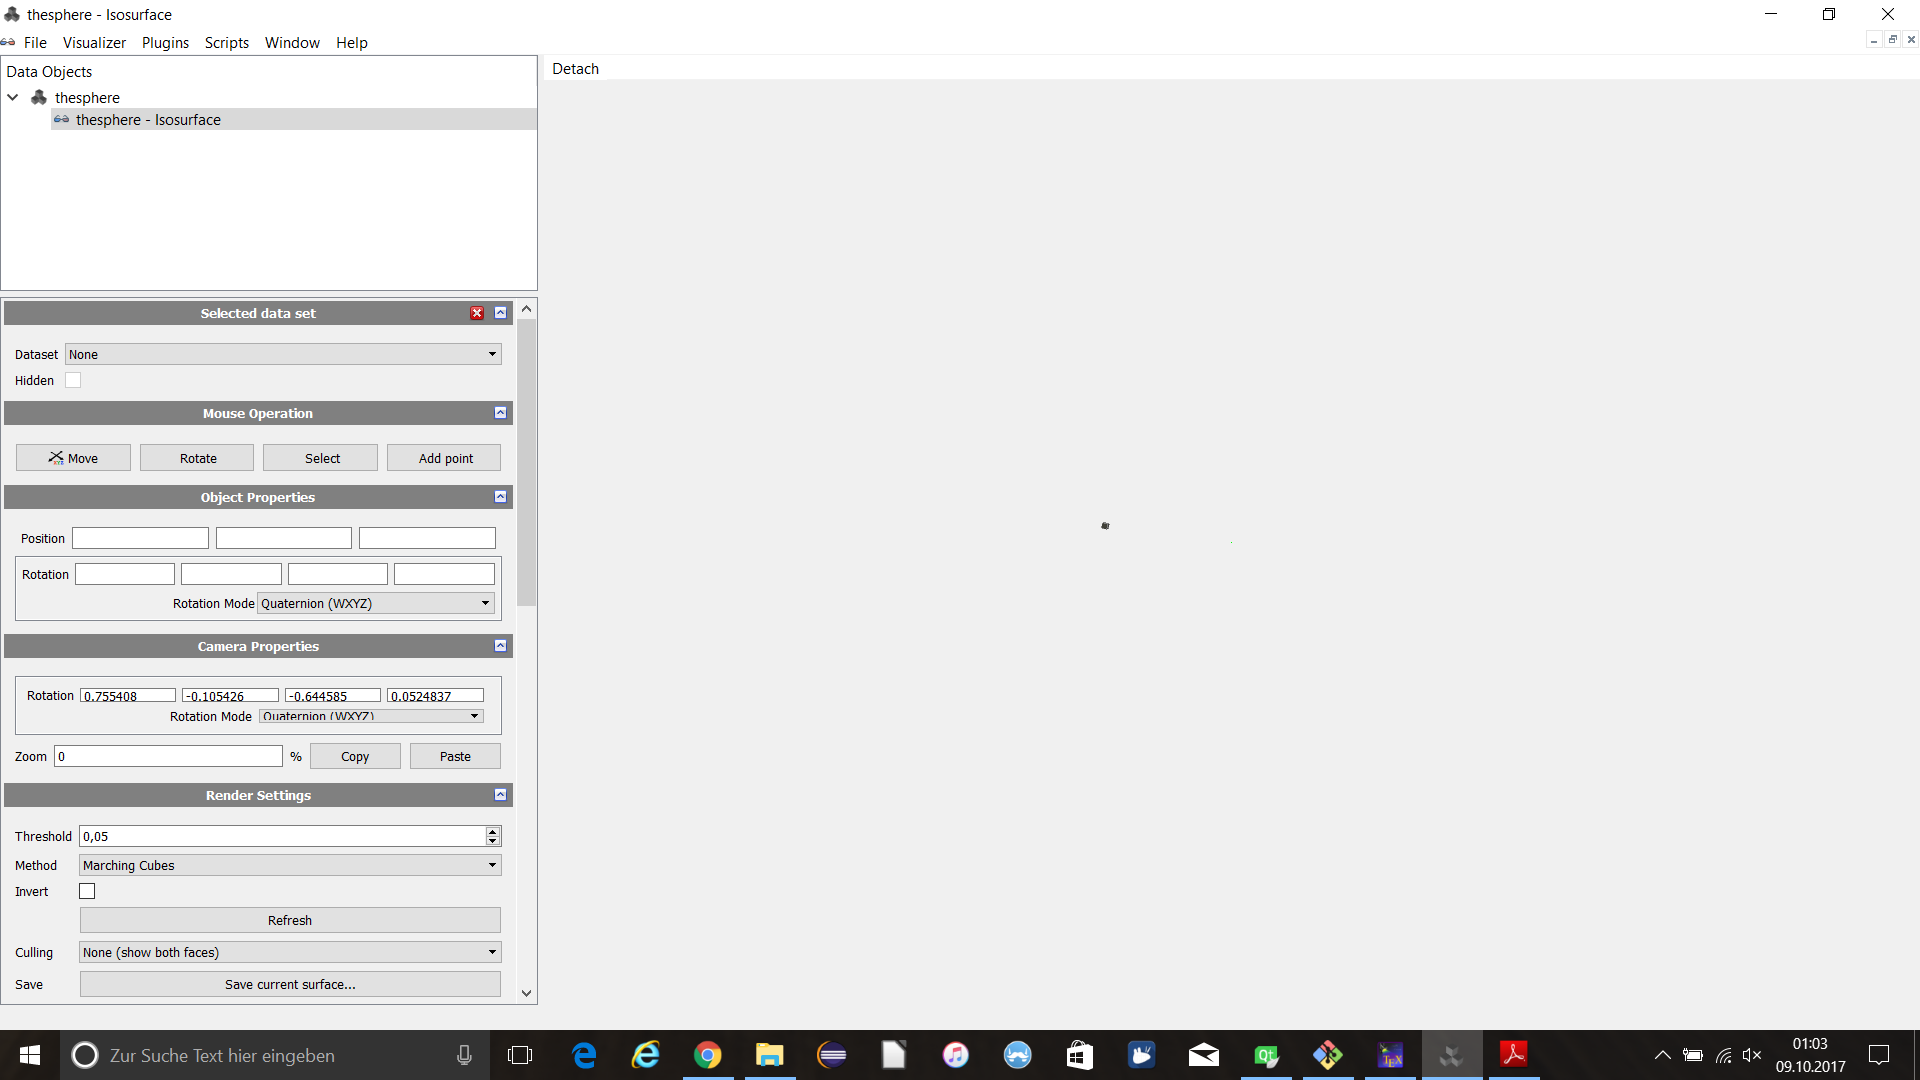
\includegraphics[width=1.0\textwidth]{img/zoomMinimum.png}
  \caption{Zoom Minimum}
\end{figure}

The maximum zoom is 100\%. It is not possible to zoom in more than 100\%.

\begin{figure}[h!]
  \centering
  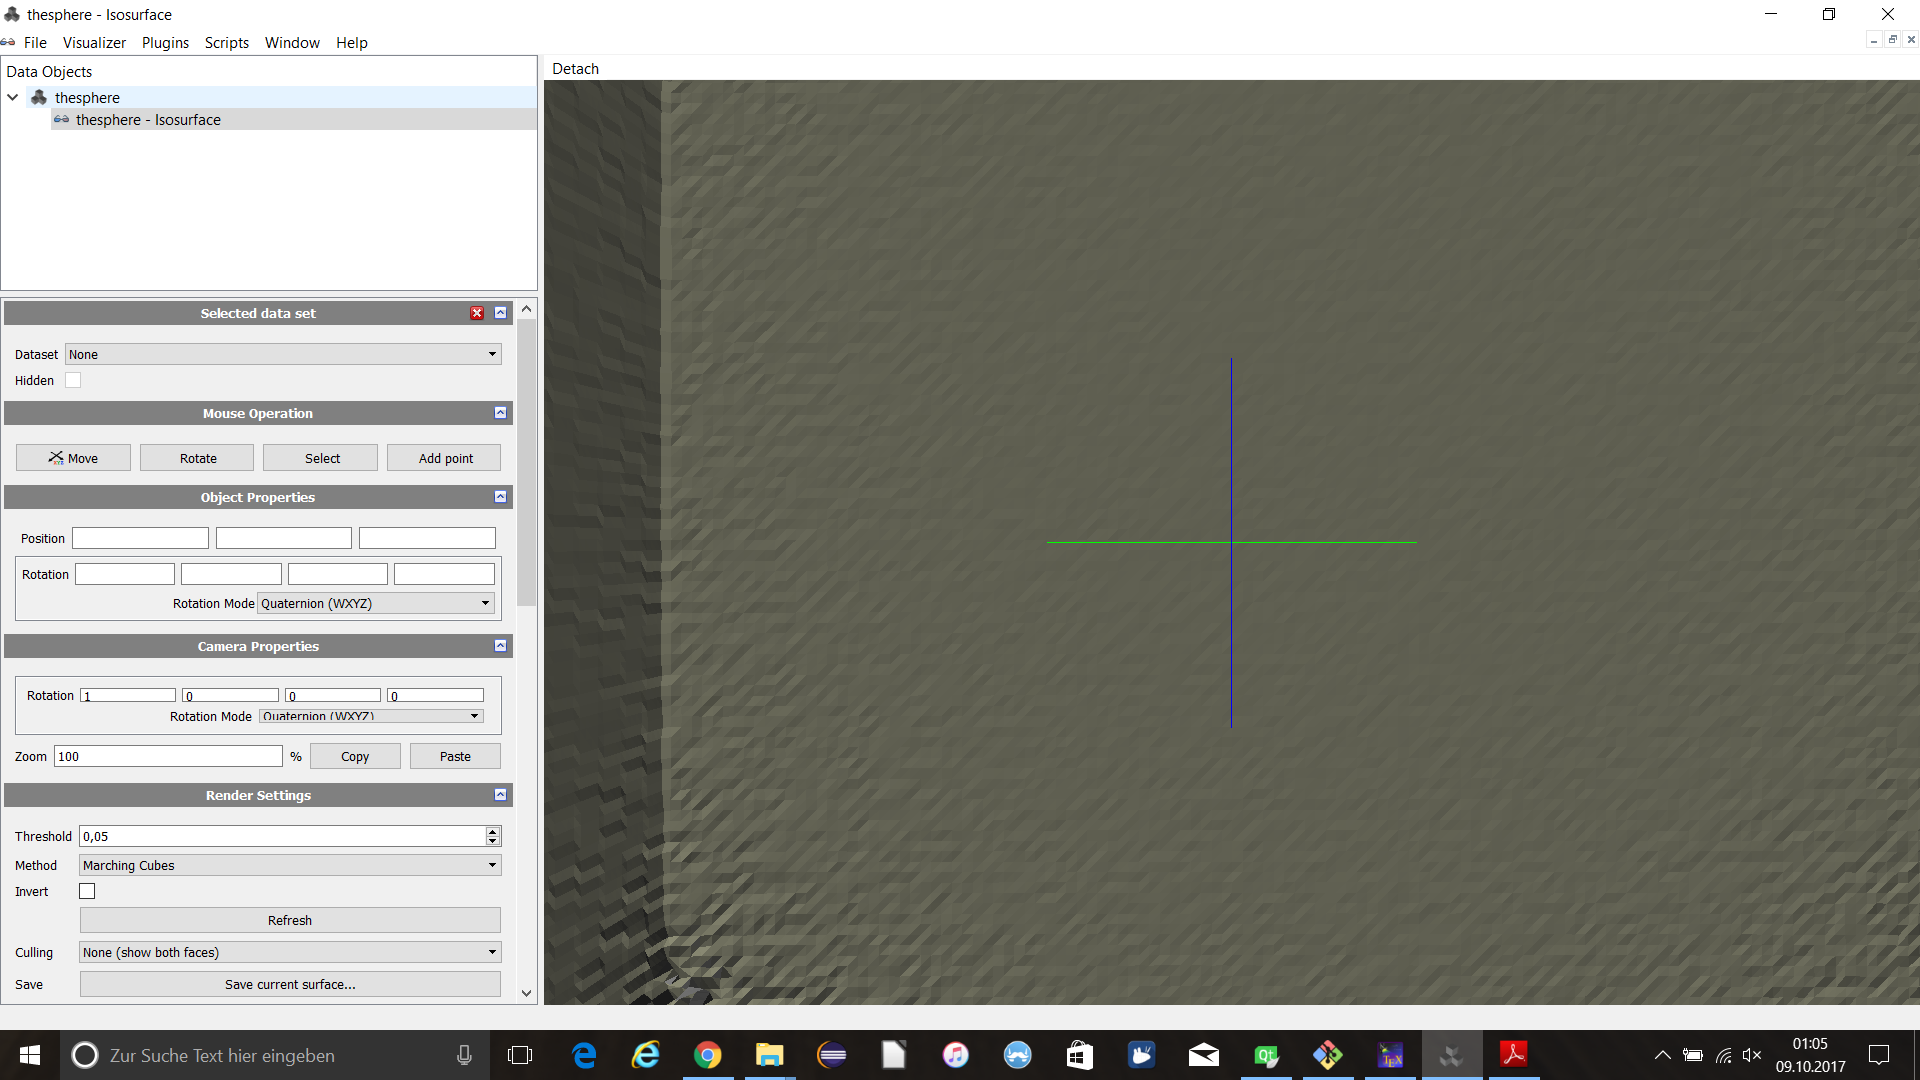
\includegraphics[width=1.0\textwidth]{img/zoomMaximum.png}
  \caption{Zoom Maximum}
\end{figure}

The default zoom when loading an object is 66.67\%.

\begin{figure}[h!]
  \centering
  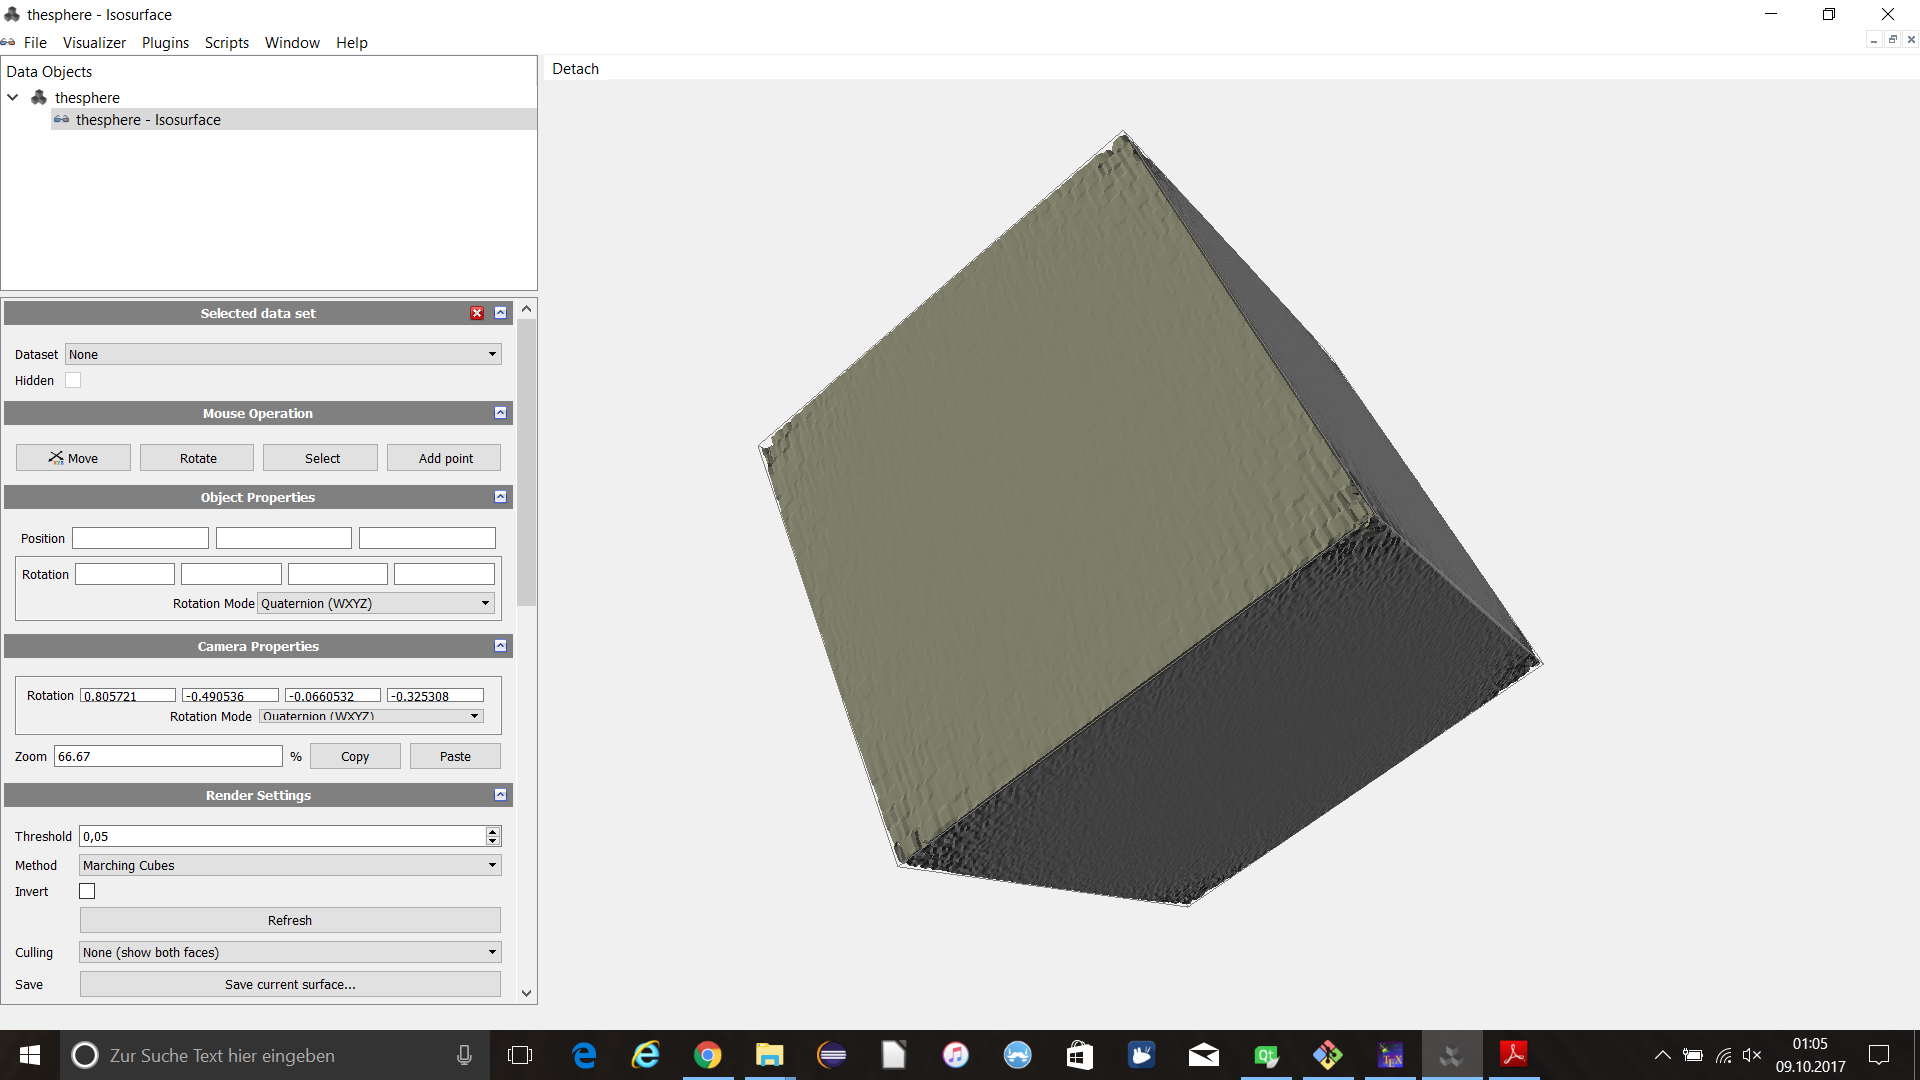
\includegraphics[width=1.0\textwidth]{img/zoomdefault.png}
  \caption{Default value of the zoom when loading a new object}
\end{figure}

\subsubsection{Copy \& Paste zoom and rotation}\label{Copy&PasteZoom&Rotation}

The zoom and rotation of the current object can be copied to the system clipboard by clicking on the \textit{copy} button, which is located directly next to the input field of the zoom.

In the same way, the zoom and rotation can be inserted from the system clipboard into the respective fields by clicking the \textit{paste} button, which is next to the \textit{copy} button.

\begin{figure}[h!]
  \centering
  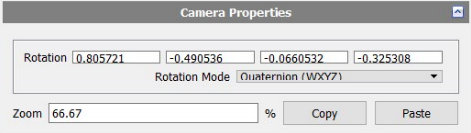
\includegraphics[width=1.0\textwidth]{img/zoomCopyAndPaste.PNG}
  \caption{Surface of copy and paste function}
\end{figure}

\newpage
\subsection{Volume Rendering}

The Volume Rendering visualizer allows seeing the data set as a whole piece. It accumulates
the voxels it finds while raycasting into the scene and thus shows the interior of
the data set.

It is useful to gather information about where specific structures are located in
the data set, if there are cavities in the data set or points with a high density.

\subsubsection{Settings}
The Volume Rendering visualizer can be set up via its side panel section.
The section has multiple options:
\begin{itemize}
  \item{\emph{Render Quality}\newline The number of samples used by the raycaster.
    Lower values are faster, higher values give more details.}
  \item{\emph{Minimum}\newline The minimum value considered as black/transparent.
    Can be used as an additional high-pass filter.}  
  \item{\emph{Maximum}\newline The maximum value considered as white/opaque.
      Can be used as a range adjustment.}
  \item{\emph{Result Scale}\newline Scales the result from the range options by
    a given amount. Can be used to tweak the image brightness.}
\end{itemize}

The settings of the visualizer are also displayed as integers to allow more precise settings.

For a computationally under-performing computer it is recommended to not use the
higher render quality settings as they draw a lot of computational power.

\subsubsection{Object Properties}

In this section current selected object properties can be seen and edited. The object responds in real time by entering in the textfields. The representation of rotation has two modes. The rotation representation of the objct can be switched beteween quaternion or euler angles by clicking on the \textit{Rotation Mode} button.

\subsubsection{Camera Properties}

The camera pooperties contains the rotation of the camera and the current relative zoom. The camera responds in real time by entering in the textfields. The Rotatin can be switched like the object properties.

\subsubsection{Restriction of the zoom}

See \ref{restrictionOfTheZoom}

\subsubsection{Copy \& Paste zoom and rotation}

See \ref{Copy&PasteZoom&Rotation}

\subsubsection{Controls}
The data set can be rotated by dragging the mouse over the visualizer window while
holding down the left mouse button.
Scrolling the mouse wheel will zoom in or out the view.

\begin{figure}[h!]
  \centering
  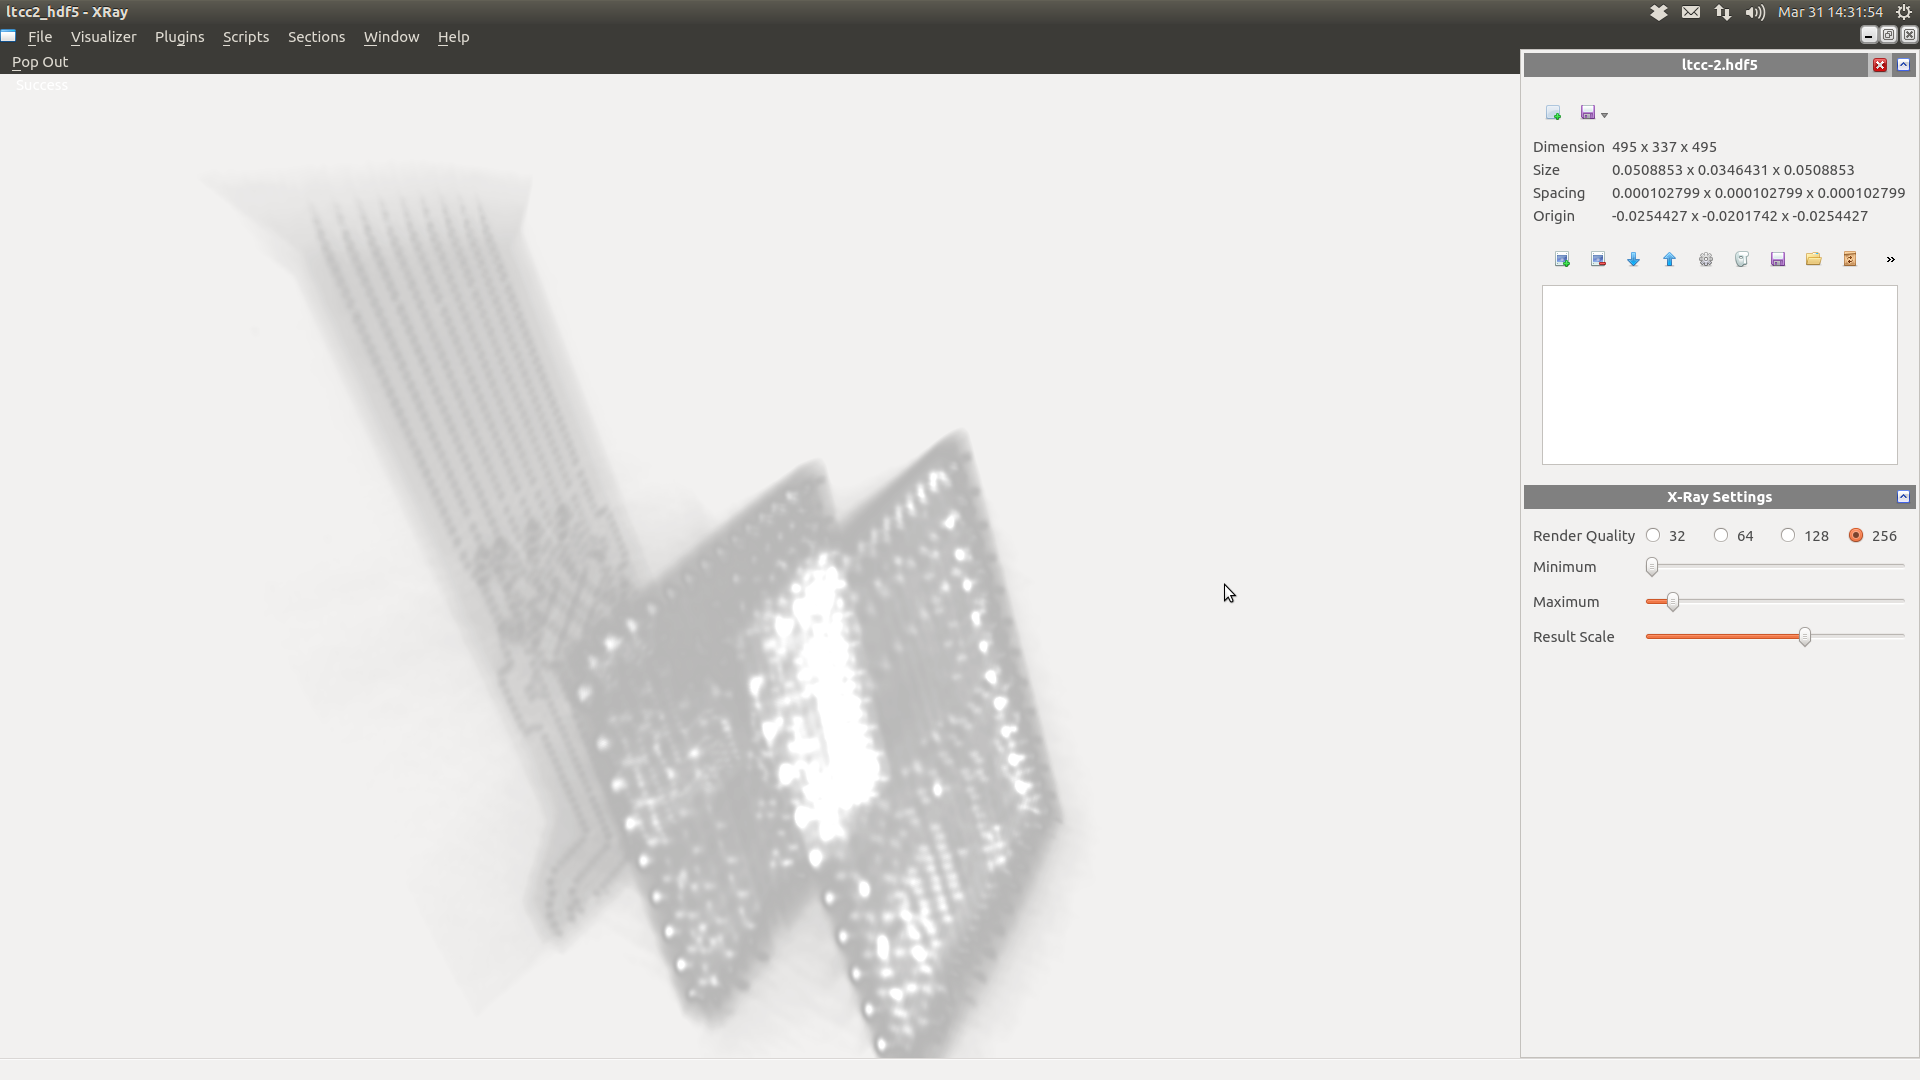
\includegraphics[width=1.0\textwidth]{img/x-ray.png}
  \caption{X-Ray}
\end{figure}
